\chapter{Design \& Specification}

As previously described, the project aims to create an extensible Lispish to JavaScript compiler. 
In order to clearly define the possible constructs for writing programs in Lispish, we need to formalise our input language. 
As Lispish defines a subset of an existing language, it is therefore even more important to be clear on what is possible and what is not. 

\section{Designing the Lispish language}\label{design-specification}

Lispish is a dynamically typed, functional language that implements a call-by-value strategy just as its superset Clojure.

The formal description of Lispish behaviour will be described using transition systems.

\subsection{Grammar of Lispish}

\begin{figure}[ht]
\centering
\begin{tabular}{ c c c }
$F$ & $\Coloneqq$ & (let \ $[x \ F]$ \ ($F$)) \\
 & $|$ & (if \ ($F$) \ $F_1$ \ $F_2$) \\
 & $|$ & (defn \ $name$ \ $[args*]$ \ ($F$)) \\
 & $|$ & (fn \ $[arg]$ \ $(F)$) \\
 & $|$ & (cond \ $(F_0)$ \ $F_1$ \ $(F_2)$ \ $F_3$) \\
 & $|$ & (recur \ $args*$) \\
 & $|$ & (let [$X$ ($(F_0)$)]  \\
 & $|$ & $T$ \\
 & $|$ & $X$ \\
 & & \\
where & & \\
 & & \\
$X$ & $\Coloneqq$ & $T$ \\
$T$ & $\Coloneqq$ & $ \ () \ \vert \ N \ \vert \ B \ \vert \ s $ \\
& & \\
operators & & \\
 & & \\
$N$ & $\Coloneqq$ & $ n \ \vert \ (op \ N \ N) $ \\
$B$ & $\Coloneqq$ & $ b \ \vert \ (bop \ t1 \ t2) \ $ \\
$op$ & $\Coloneqq$ & $ \ + \ \vert \ - \ \vert \ * \ \vert \ / \ \vert \ < \ \vert \ > \ \vert \ =$\\
$bop$ & $\Coloneqq$ & $ \ and \ \vert \ or \ \vert \ not$ \\
& & \\
atomic & & \\
 & & \\
$s$ & $\Coloneqq$ & $ String $ \\
$n$ & $\Coloneqq$ & $ Integer $ \\
$b$ & $\Coloneqq$ & $ true \ \vert \ false $ \\
$()$ & $\Coloneqq$ & $ List $ \\
\end{tabular}
\texttt{*} denotes multiple arity 

\caption{Lispish grammar}
\label{fig:lispish-grammar}
\end{figure}

Figure ~\ref{fig:lispish-grammar} contains the Lispish grammar. The grammar of the language formally defines the legal operators and operations that the language provides for writing programs in Lispish.

\subsection{Evaluation relations (Big-Step Semantics)}

Figure ~\ref{fig:lispish-big-step} describes the evaluation relations of Lispish. These relations therefore describe the constructs that can be used when writing Lispish programs. They, however, do not relate to the evaluation relations of the generated JavaScript code. 

% TODO figure layout
\begin{figure}[ht]
\centering
Opertors:\
\[
\inference[bop]{E_1, s \ $$\Downarrow$$ \ b_1, s' \ E_2, s' \ $$\Downarrow$$ \ b_2, s''}
{(bop \ E_1 \ E_2) \ $$\Downarrow$$ \ b, s'', if (= b \ (bop \ b_1 \ b_2))}
\]
\[
\inference[op]{E_1, s \ $$\Downarrow$$ \ n_1, s' \ E_2, s' \ $$\Downarrow$$ \ n_2, s''}
{(op \ E_1 \ E_2) \ $$\Downarrow$$ \ b, s'', if (= b \ (op \ n_1 \ n_2))}
\] \\

\vspace*{15pt}
Atomic: \
\[
\inference[String]{}
{s \ $$\Downarrow$$ \ s}
\]
\[
\inference[Integer]{}
{n \ $$\Downarrow$$ \ n}
\]
\[
\inference[List]{n \ $$\Downarrow$$ \ v}
{(n) \ $$\Downarrow$$ \ v}
\]

\vspace*{15pt}
Forms (F): \
\[
\inference[let]{t_0 \ $$\Downarrow$$ \ v}
{(\text{let } \ {[x \ (t_0)]} \ (t_1)) \ $$\Downarrow$$ \ t_1 {[}x \ $$\mapsto$$ \ v{]} }
\]
\[
\inference[if true]{{t_0} \ $$\Downarrow$$ \ \textsc{True} & t_1 \ $$\Downarrow$$ \ v}
{(if \ (t_0) \ t_1 \ t_2) \ $$\Downarrow$$ \ v) }
\]
\[
\inference[if false]{t_0 \ $$\Downarrow$$ \ \textsc{False} & t2 \ $$\Downarrow$$ \ v}
{(if \ (t_0) \ t_1 \ t_2) \ $$\Downarrow$$ \ v) }
\]
\[
\inference[cond]{t_0 \ $$\Downarrow$$ \ \textsc{False} & t_1 \ $$\Downarrow$$ \ \textsc{True} & t_3 \ $$\Downarrow$$ \ v}
{(cond \ (t_0) \ t_2 \ (t_1) \ t_3) \ $$\Downarrow$$ \ v) }
\]
\[
\inference[defn]{ {t_0 \ [x]} \ $$\Downarrow$$ \ v}
{(defn \ s \ {[x]} \ (t_0)) \ $$\Downarrow$$ \ s \ $$\mapsto$$ \ v }
\]
\[
\inference[fn]{ {t_0 \ [x]} \ $$\Downarrow$$ \ v}
{(fn \ {[x]}  \ (t_0) \ $$\Downarrow$$ \ v }
\]
\[
\inference[call to external function]{ {args*} \ $$\Downarrow$$ \ v}
{(s \ {args*}) \ $$\Downarrow$$ \ v }
\]
\[
\inference[recur]{ {args*} \ $$\Downarrow$$ \ v}
{(recur \ {args*}) \ $$\Downarrow$$ \ v }
\]\vspace*{10pt}

Recur emits all of its arguemnts and provides it as arguments to JavaScript 
\texttt{arguments.callee(args*)} function. \\
The \texttt{(s )} form that uses a string as a function, allows for invoking named function recursively, as well as any in-built JavaScript functions and library (e.g. jQuery) functions, as described in ~\ref{DOM}.
\caption{Lispish evaluation relations (Big-Step Semantics)}
\label{fig:lispish-big-step}
\end{figure}

\section{Development methodology}
In order to streamline the process of developing the compiler, I have decided to use the Test Driven Development (TDD) methodology that emphasizes building small units of functionalities that can be individually tested by unit tests. 

Clojure allows developers to create programs using the REPL (Read Evaluation Print Loop), which is a characteristic feature in modern dynamic programming languages. It allows you to write your functions, evaluate them and get an instant result from an interpreter that interacts with your code. This reduces the amount of unit tests that have to be implemented for trivial functions in a TDD project. 

% TODO
A REPL is a great resource not only for the rapid development and function prototyping, but also ensuring that they yield the correct results before the project as a whole is compiled.

\section{Compiling Lispish to JavaScript}

\subsection{Compilation Pipeline}

\begin{figure}[!H]
	\begin{center}
	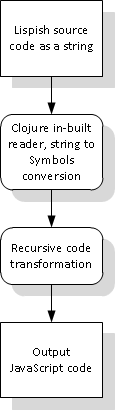
\includegraphics{Graphics/abstract_compilation.png}
	\caption[Abstract compilation of Lispish to JavaScript.]
   {Abstract compilation of Lispish to JavaScript.}
	\end{center}
  \label{fig:abstract-compilation}
\end{figure}


The compiler in its simplest form will perform a one-to-one translation from Lispish to JavaScript. 

% TODO
The input source will be treated by the Clojure reader will prevent the code from being evaluated and it will pass it along down the pipeline to its respective emitters as illustrated on figure ~\ref{fig:abstract-compilation}. Code will be treated as data and I will use the prefix notation to my advantage, treating each expression as its respective node in a parse tree. 

\subsection{Clojure Homoiconicity and Using clojure.reader as a Parser}
Clojure is a homoiconic language, meaning that the code itself is described in terms of data structures that the language understands (s-expression forms, lists and in-built data structures). It comes bundled with a Clojure reader \cite{clojure.reader} that can parse the text source file into objects of specific Clojure type. Those objects are essentially Clojure data structures that then are treated by the Clojure compiler and similarly in case of Lispish will be treated by the translator program, to generate corresponding JavaScript code. 

As pointed out in the referenced \cite{clojure.reader} section of the Clojure documentation, the Clojure reader is represented by the \texttt{(reader )} function, that takes text as an input and produces the object represented by that text. 
This is also the entry point of our translator, as illustrated on ~\ref{fig:abstract-compilation} as the entry block in the flowchart. 
The translator will then generate different JavaScript constructs based on the type of the object that it comes across when recursively evaluating the type of each nested expression. 
